\chapter{Dataset}
\label{ch:dataset}

\section{Dataset Selection}
\label{sec:dataset-selection}

The main dataset used in this project is Cochrane-auto~\cite{bakker2024cochraneauto}, an aligned corpus that pairs sentences from Cochrane systematic review abstracts with their official plain-language summaries. It was chosen over general-domain simplification datasets because it puts the project's central question, whether a model can simplify health text without losing medical substance, directly at the centre of the training data rather than treating it as an afterthought.

ASSET and WikiAuto were considered as alternatives but kept to a supporting role. ASSET is a multi-reference sentence simplification dataset built from encyclopaedic text, useful for understanding how evaluation against multiple references works, but not representative of clinical writing~\cite{alvamanchego2020asset}. WikiAuto is similarly built on Wikipedia-style prose and carries stylistic habits that do not transfer cleanly to patient-facing health content~\cite{jiang2020wikiauto}. Both remain useful as comparison points rather than as training data for this project.

\section{Acquisition}
\label{sec:acquisition}

Cochrane-auto is distributed with the code used to build it, together with pre-computed sentence-level, paragraph-level, and document-level versions of the aligned data, already split into training, validation, and test sets. This project uses the published split throughout rather than constructing a new one, both to avoid accidentally leaking test examples into training and to keep any later comparison against the original paper straightforward.

Modelling in this project works at sentence level. Cochrane abstracts and their lay summaries can run to several hundred words, and full paragraph or document-level training would demand longer sequence lengths and considerably more compute than a project of this scale can commit to. Sentence-level pairs keep the task tractable for a compact model such as T5-small while still capturing the core rewriting behaviour this project is interested in.

\section{Structure of the Aligned Data}
\label{sec:data-structure}

Each row in the sentence-level data links one sentence from a technical abstract to zero or more sentences from the corresponding lay summary. Every row carries a label describing the type of rewrite that connects the two, produced by the alignment model used to build Cochrane-auto. \Cref{tab:alignment-labels} summarises what each label means and how it was used in this project.

\begin{table}[htbp]
    \centering
    \caption{Rewrite-operation labels in the Cochrane-auto sentence-level data.}
    \label{tab:alignment-labels}
    \begin{tabular}{@{}ll@{}}
        \toprule
        \textbf{Label} & \textbf{Meaning} \\
        \midrule
        \texttt{rephrase} & The technical sentence maps to a single simplified sentence. \\
        \texttt{split} & Its content is spread across more than one simplified sentence. \\
        \texttt{merge} & It is combined with other sentences into one simplified sentence. \\
        \texttt{delete} & The sentence was dropped entirely from the lay summary. \\
        \texttt{ignore} / \texttt{none} & No reliable alignment could be established. \\
        \bottomrule
    \end{tabular}
\end{table}

Training pairs for this project were built from every row with a non-empty simplified target, which naturally keeps \texttt{rephrase} and \texttt{split} rows and the contributing row of a \texttt{merge} group, while correctly leaving out sentences that were deleted or never reliably aligned. In the training split, 5{,}239 sentences were tagged \texttt{rephrase}, 521 \texttt{split}, and 365 \texttt{merge}, against 4{,}063 tagged \texttt{delete} and 1{,}322 tagged \texttt{ignore} or \texttt{none}. \Cref{fig:label-distribution} shows how these counts break down across the training, validation, and test splits.

\begin{figure}[htbp]
    \centering
    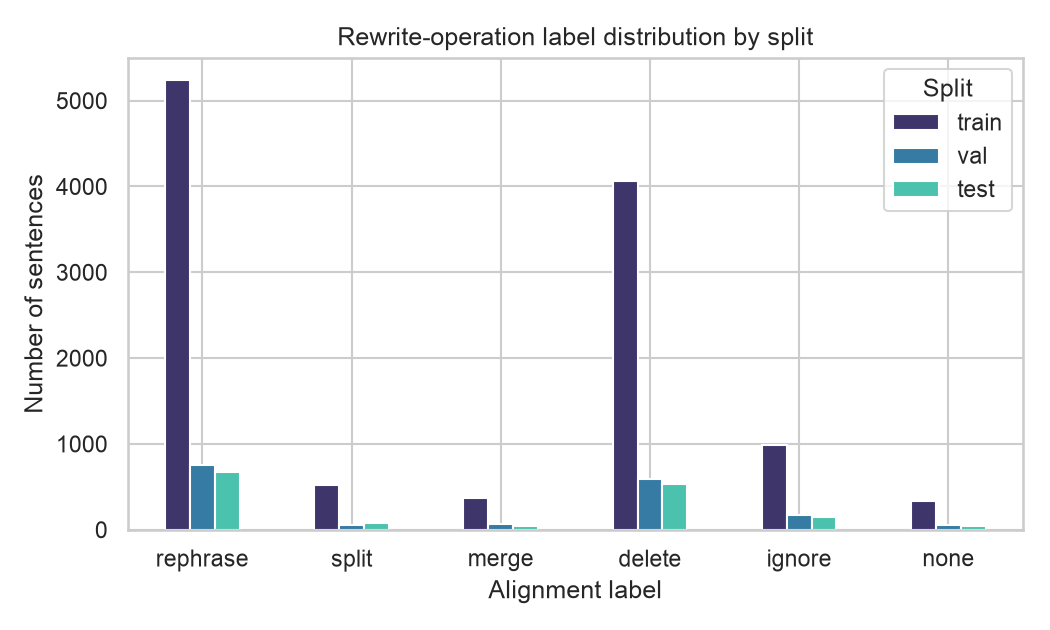
\includegraphics[width=0.85\textwidth]{figures/01_label_distribution.png}
    \caption{Rewrite-operation label distribution across the train, validation, and test splits.}
    \label{fig:label-distribution}
\end{figure}

\section{Exploratory Analysis}
\label{sec:eda}

Before any modelling took place, the extracted pairs were examined for sentence length, the degree to which the simplified version compresses or expands the original, and a manual reading of a sample from each label category. This step matters beyond simple description: it shapes what counts as a fair baseline and what kind of model error is worth taking seriously later in the project.

\Cref{tab:eda-summary} reports descriptive statistics for the 7{,}082 training pairs with a non-empty simplified target. The compression ratio is the simplified sentence's word count divided by the complex sentence's word count, so a value below one means the plain-language version is shorter.

\begin{table}[htbp]
    \centering
    \caption{Descriptive statistics for training pairs (word counts and compression ratio).}
    \label{tab:eda-summary}
    \begin{tabular}{@{}lrrr@{}}
        \toprule
         & \textbf{Complex (words)} & \textbf{Simple (words)} & \textbf{Compression ratio} \\
        \midrule
        Mean   & 24.86 & 23.59 & 1.13 \\
        Std.\ dev. & 15.66 & 12.88 & 0.72 \\
        Minimum & 1     & 3     & 0.06 \\
        25th percentile & 15 & 15 & 0.73 \\
        Median & 21    & 21    & 1.00 \\
        75th percentile & 31 & 29 & 1.27 \\
        Maximum & 186   & 145   & 9.75 \\
        \bottomrule
    \end{tabular}
\end{table}

The mean compression ratio of 1.13 is higher than intuition might suggest for a simplification dataset, and it points to something worth stating plainly. Cochrane lay summaries do not only shorten technical sentences. In a meaningful share of cases they are about the same length or longer than the source, because the writer has added context, defined a term, or explained why a result matters rather than simply trimming it. \Cref{fig:length-compression} shows the full length distributions and the spread of compression ratios, and \cref{fig:complex-vs-simple} plots complex sentence length against simplified sentence length directly, coloured by rewrite label.

\begin{figure}[htbp]
    \centering
    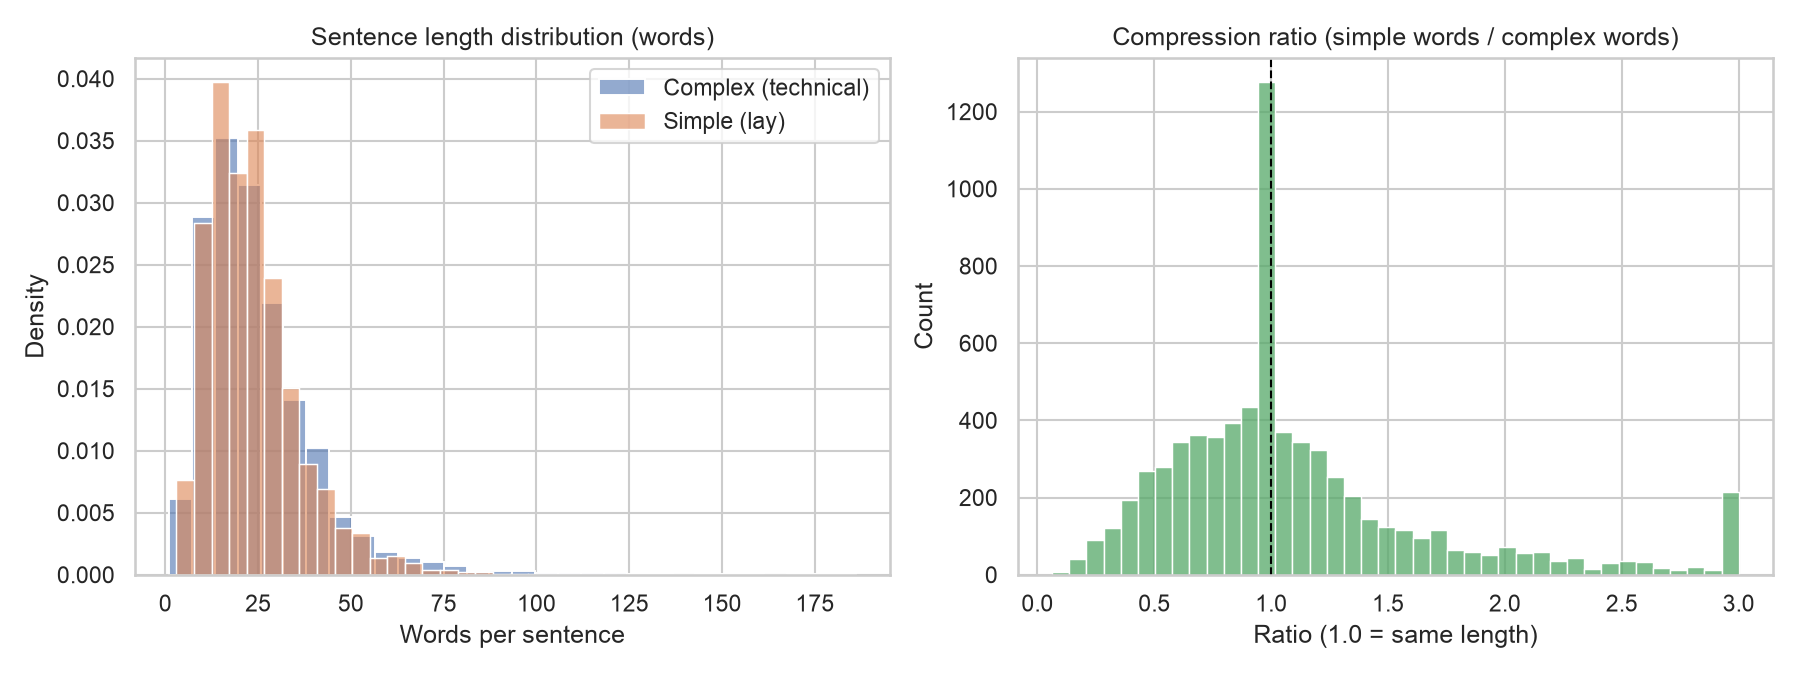
\includegraphics[width=\textwidth]{figures/02_length_and_compression.png}
    \caption{Sentence length distributions for complex and simplified text (left) and the distribution of compression ratios (right).}
    \label{fig:length-compression}
\end{figure}

\begin{figure}[htbp]
    \centering
    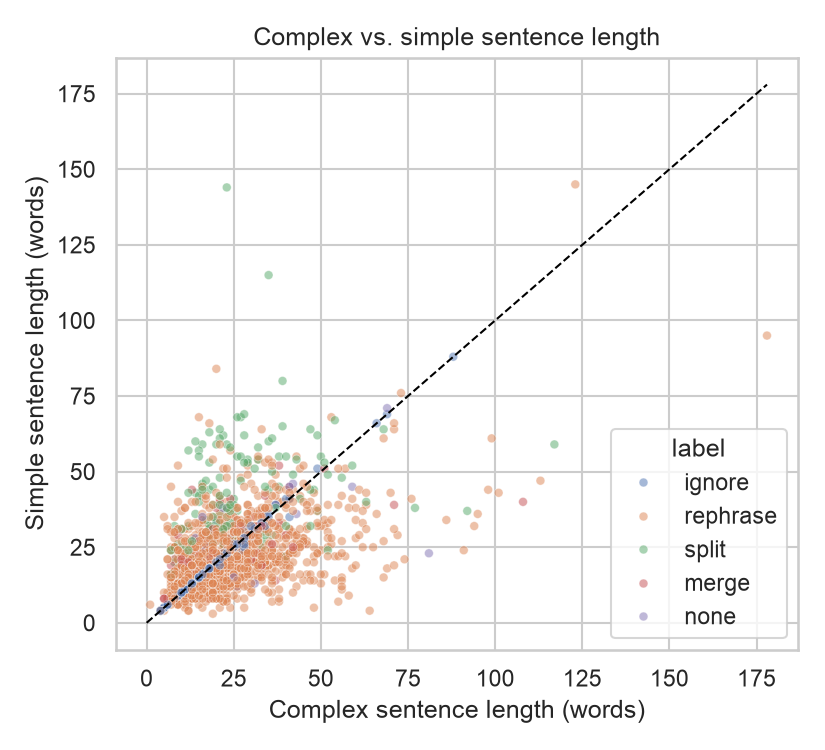
\includegraphics[width=0.75\textwidth]{figures/03_complex_vs_simple_scatter.png}
    \caption{Complex sentence length plotted against simplified sentence length, by rewrite-operation label.}
    \label{fig:complex-vs-simple}
\end{figure}

A manual reading of sample pairs from each label category reinforced this observation. Several \texttt{rephrase} pairs read as a fairly direct restatement, but a number of \texttt{split} pairs showed the lay summary adding a sentence of explanation that has no direct counterpart in the source text at all, of the kind ``this means the results should be interpreted with caution.'' That pattern suggests the task learned from this dataset is not pure sentence simplification in the narrow sense. It sits closer to a constrained form of lay summarisation, where the model is expected to compress, clarify, and occasionally explain, all within a single rewrite. That framing carries through the rest of this thesis, including the discussion of results in \cref{ch:results-discussion}, where some of the model's apparent underperformance turns out to reflect this mismatch between what the source sentence says and what the reference summary was actually written to communicate.
